\subsection{Exemple du Bitcoin}
\framewithtitle{Exemple du Bitcoin}

\begin{frame}{Bitcoin : décentralisation}
  \begin{columns}
    \begin{column}{0.6\textwidth}
      \begin{itemize}
        \item La blockchain Bitcoin est un réseau peer-to-peer décentralisé
        \item Le réseau Bitcoin \textbf{toujours en ligne} (tant qu'il y a des noeuds)
        \item Pas d'administration centrale (donc pas de Bitcoin Corp. Limited)
        \item Tout individu peut y participer en créant un \textquote{n\oe{}ud} = démarrer un logiciel en CLI
      \end{itemize}
    \end{column}

    \begin{column}{0.4\textwidth}
      \begin{figure}
  \resizebox{\columnwidth}{!}{%
    \begin{tikzpicture}[font=\sffamily\footnotesize,
        Node/.style={shape=ellipse,draw}
      ]

      \node[Node] (N_A) at (0,0) {Node A};
      \node[Node, above right=2cm and 2cm of N_A] (N_B) {Node B};
      \node[Node, below right=2cm and 2cm of N_A] (N_C) {Node C};
      \node[Node, above left=2cm and 2cm of N_A] (N_D) {Node D};
      \node[Node, below left=2cm and 2cm of N_A] (N_E) {Node E};

      \draw[<->] (N_A) -- (N_B);
      \draw[<->] (N_A) -- (N_C);
      \draw[<->] (N_A) -- (N_D);
      \draw[<->] (N_A) -- (N_E);
      \draw[<->] (N_D) -- (N_E);
      \draw[<->] (N_D) -- (N_B);
      \draw[<->] (N_C) -- (N_E);
      \draw[<->] (N_C) -- (N_B);
    \end{tikzpicture}%
  }

  \caption{Réseau peer-to-peer}
\end{figure}
    \end{column}
  \end{columns}
\end{frame}

\begin{frame}[fragile]{Bitcoin : livre de comptes}
  \begin{columns}
    \begin{column}{0.05\textwidth}
    \end{column}

    \begin{column}{0.65\textwidth}
      La blockchain Bitcoin est un système décentralisé permettant aux utilisateurs d'échanger une monnaie numérique, le Bitcoin.

      \begin{itemize}
        \item Les Bitcoin (BTC) sont stockés dans des comptes, identifiés par une adresse
        \item L'ensemble des soldes des comptes, le \textquote{livre de comptes} est stocké à de multiples endroits
        \item Tout individu peut obtenir un compte gratuitement (on en parle plus tard)
        \item Envoyer des $x$ BTC d'une adresse $a$ à une adresse $b$ revient à faire
      \end{itemize}

      \begin{minted}{solidity}
        solde_a -= x; solde_b += x
      \end{minted}
    \end{column}

    \begin{column}{0.2\textwidth}
      \begin{table}[]
  \begin{tabularx}{\textwidth}{X|l}
    \toprule
    Compte & Solde \\ \midrule
    0001   & 12    \\
    0002   & 3.42  \\
    0003   & 4.4   \\
    0004   & 3.6   \\
    0005   & 5     \\
    \vdots &       \\
    1232   & 30.45 \\
    1233   & 0.34  \\
    1234   & 113.3 \\
    1235   & 4.97  \\ \bottomrule
  \end{tabularx}
\end{table}
    \end{column}

    \begin{column}{0.1\textwidth}
    \end{column}
  \end{columns}
\end{frame}

\begin{frame}{Bitcoin : opérer un node}
  \begin{columns}
    \begin{column}{0.5\textwidth}
      \begin{itemize}
        \item Opérer un node = particper à la blockchain = augmenter la décentralisation
        \item \textquote{Relativement léger} : 2 Go de RAM, 7 Go de disque, connexion 400 kilobits/sec
        \item Attention, certains pays interdisent d'opérer un node : Afghanistan, Algérie, Bangladesh, Bolivie, Chine, Égypte, Kosovo, Maroc, Népal
      \end{itemize}
    \end{column}

    \begin{column}{0.5\textwidth}
      \begin{figure}
  \resizebox{\textwidth}{!}{
    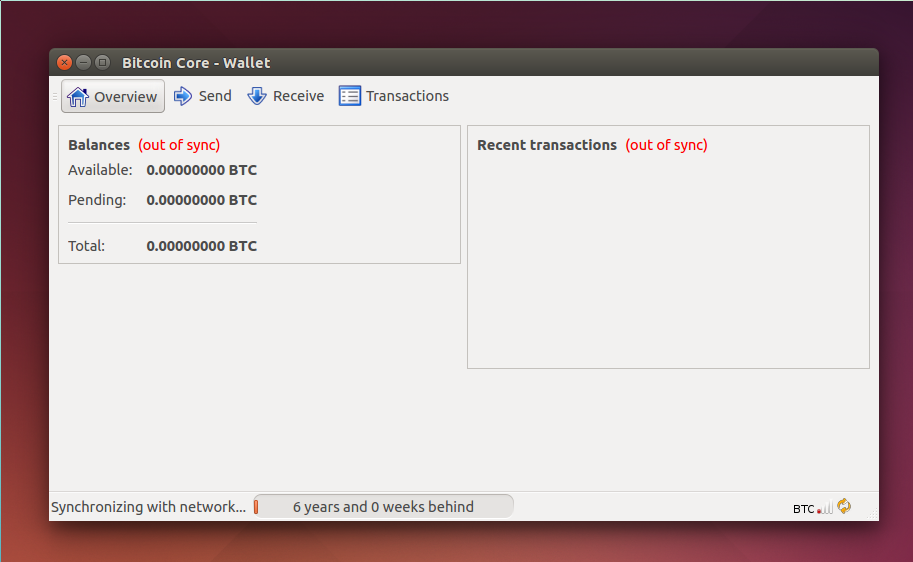
\includegraphics{img/btc-core-gui.png}
  }
  \caption{Bitcoin Core GUI}
  \label{fig:btc-core-gui}
\end{figure}
    \end{column}
  \end{columns}
\end{frame}

\begin{frame}{Bitcoin : créer un compte}
  \begin{itemize}
    \item La blockchain Bitcoin, comme la majorité des blockchain, fonction avec un couple de clé publique/privée.
    \item Chaque clé privée donne accès à un compte (=adresse) de la blockchain.
    \item Attention, si \textbf{la clé privée fuite, le compte est définitivement compromis}.
  \end{itemize}

  Exemple avec \url{https://iancoleman.io/bip39/} :

  \begin{itemize}
    \item Clé privée \texttt{Kwp24SX6Uo1xNUDihM3oeSmg9MHrPm9ZEp7v26jrmxMmC5js4i5f}
    \item Clé publique \texttt{0256fa0a8c520a0a501000845ebaf112295b3c5c29b4b0f7b2d01b933451d9ebf8}
    \item Adresse \texttt{1CLHPJK9Z1NFzvQSnP5CozanMo5L35Caq1}
  \end{itemize}
\end{frame}

\begin{frame}{Bitcoin : effectuer une transaction}
  \begin{block}{Définition : transaction}
    Sur la blockchain Bitcoin, une transaction est un message signé (avec la clé privée) par un utlisateur de blockchain.
    Elle contient les informations suivantes :

    \begin{itemize}
      \item L'adresse de l'émetteur.
      \item L'adresse du destinataire.
      \item La valeur (=montant) de la transaction.
    \end{itemize}
  \end{block}
\end{frame}

\begin{frame}{Bitcoin : effectuer une transaction}
  Exemple : Alice, qui possède 10 BTC, peut en envoyer 1 BTC à Bob en signant le message suivant :
  \textquote{Moi, Alice, envoie 1 BTC à Bob}

  Une fois la transaction signée, il faut l'envoyer au réseau Bitcoin.
  Pour cela, Alice doit enoyer la transaction à un node Bitcoin.

  Ce dernier va alors vérifier la transaction (si la signature est valide) et si c'est le cas, l'enoyer à d'autres noeuds du réseau, qui vont eux-mêmes vérifier la transaction, etc.
  Par effet boule de neige, la transaction fini par atteindre rapidement tous les noeuds Bitcoin.
\end{frame}

\begin{frame}{Bitcoin : effectuer une transaction}
  \begin{figure}
  \resizebox{\columnwidth}{!}{%
    \begin{tikzpicture}[
        Node/.style={draw}
      ]
      % Actors
      \node[label=Alice] (alice) at (0,0) {
\includegraphics[height=4cm]{img/alice.png}};
      \node[draw,right = 1cm of alice] (tx) {Transaction};

      \node[Node,right = 9cm of alice] (n1) {Node 1};
      \node[Node,above right = 1cm and 2cm of n1] (n2) {Node 2};
      \node[Node,left = 1cm of n1] (n3) {Node 3};
      \node[Node,below right = 2cm and 1cm of n1] (n4) {Node 4};
      \node[Node,above left = 1cm and 0.5cm of n1] (n5) {Node 5};
      \node[Node,below left = 2cm and 1cm of n1] (n6) {Node 6};
      \node[Node,below = 1cm of n1] (n7) {Node 7};
      \node[Node,left = 3cm of n1] (n8) {Node 8};

      \draw[->] (alice) -- (tx) -- (n8);
      \foreach \node in {n5,n3,n6}
      \draw[->] (n8) -- (\node);
      \foreach \node in {n1,n7,n2}
      \draw[->] (n5) -- (\node);
      \foreach \node in {n1,n7}
      \draw[->] (n3) -- (\node);
      \foreach \node in {n1,n7,n4}
      \draw[->] (n6) -- (\node);

    \end{tikzpicture}%
  }

  \caption{Diffusion ou \textquote{broadcast} d'une transaction}
\end{figure}
\end{frame}

\begin{frame}{Bitcoin : problème du consensus}
  \begin{itemize}
    \item Dans le schéma précédent, Alice a initialiement envoyé sa transaction au Node 8, ce qui implique que celui-ci a eu temporairement une liste de transactions différente des autres nodes.
    \item En parallèle, d'autres individus envoient des transactions à d'autres nodes.
    \item En pratique, aucun node n'a exactement la même liste de transactions.
    \item[$\Rightarrow$] C'est le problème du consensus = dans un système décentralisé, commet faire en sorte de mettre tout le monde d'accord ?
  \end{itemize}
\end{frame}

\begin{frame}[fragile]{Bitcoin : structure en blocs}
  \begin{columns}
    \begin{column}{0.5\textwidth}
      \begin{block}{Définition : bloc}
        Dans une blockchain, un bloc est un ensemble de transactions.
      \end{block}

      \begin{itemize}
        \item Dans la blockchain Bitcoin, la taille d'un bloc est limité à 1 MB ce qui correspond à environ 2000 transactions.
      \end{itemize}
    \end{column}

    \begin{column}{0.5\textwidth}
      \begin{figure}
  \begin{minted}{text}
    Block #4598794

    Alice sends 10 BTC to Bob
    John sends 5 BTC to Alfred
    Juliette sends 3 BTC to Mathieu
    Bob sends 3 BTC to Mathieu
    Mathieu sends 4 BNTC to John

    Nonce 90348953a8df7fe9
  \end{minted}

  \caption{Exemple textuel d'un bloc}
\end{figure}
    \end{column}
  \end{columns}
\end{frame}

\begin{frame}{Bitcoin : consensus par preuve de travail \textquote{proof-of-work}}

  \begin{columns}
    \begin{column}{0.5\textwidth}
      \begin{itemize}
        \item Afin d'obtenir le consensus, Satoshi Nakamoto a choisi d'utiliser la preuve de travail ou \textquote{proof-of-work}.
        \item Afin de proposer son bloc, le node doit résoudre un problème cryptographique difficile : il doit réussir à concevoir un bloc dont le hash avec l'algorithme SHA-256 commence par un certain nombre de zéro.
        \item Pour cela, le node fait varier le \textbf{nonce} du bloc, qui est un text arbitraire ajouté en fin de bloc.
      \end{itemize}

    \end{column}

    \begin{column}{0.5\textwidth}
      \begin{figure}
  \begin{minted}{text}
    Block #4598794

    Alice sends 10 BTC to Bob
    John sends 5 BTC to Alfred
    Juliette sends 3 BTC to Mathieu
    Bob sends 3 BTC to Mathieu
    Mathieu sends 4 BNTC to John

    Nonce 90348953a8df7fe9
  \end{minted}

  \caption{Exemple textuel d'un bloc}
\end{figure}
    \end{column}
  \end{columns}
\end{frame}

\begin{frame}{Bitcoin : consensus par preuve de travail \textquote{proof-of-work}}
  \begin{columns}
    \begin{column}{0.5\textwidth}
      \begin{itemize}
        \item Si le node trouve la solution, il doit la diffuser au reste du réseau qui vérifieront le nonce trouvé.
        \item En récompense, le node reçoit 6.25 BTC soit environ 150000€ au 14 mai 2023.
        \item La seule manière de trouver la solution est la force brute (cf. sécurité des fonctions de hachage).
        \item On appelle également les nodes \textquote{mineurs}.
        \item Un bloc est miné toutes les 10 minutes.
      \end{itemize}

    \end{column}

    \begin{column}{0.5\textwidth}
      \begin{figure}
  \begin{minted}{text}
    Block #4598794

    Alice sends 10 BTC to Bob
    John sends 5 BTC to Alfred
    Juliette sends 3 BTC to Mathieu
    Bob sends 3 BTC to Mathieu
    Mathieu sends 4 BNTC to John

    Nonce 90348953a8df7fe9
  \end{minted}

  \caption{Exemple textuel d'un bloc}
\end{figure}
    \end{column}
  \end{columns}
\end{frame}

\begin{frame}{Bitcoin : aspect économiques et halving}
  \begin{itemize}
    \item Sachant que chaque bloc miné introduit des nouveaux bitcoin dans le marché, la valeur du bitcoin baisse nécessairement sur la durée (plus de bitcoin=moins de valeur pour 1 bitcoin).
    \item Ce phénomène est comparable à l'inflation des monnaies traditionnelles.
  \end{itemize}

  \begin{block}{Halving (de l'anglais \textit{half}, moitié)}
    Dans la blockchain Bitcoin, les récompenses de bloc sont divisées par deux tous les 210000 blocs, soit environ 4 ans.
    En 2009, un bloc valait 50 BTC, en 2013 25 BTC, en 2016 12 BTC et en 2020 6.25 BTC.
  \end{block}

  \begin{block}{Maximum supply}
    Dû au mécanisme de halving, il ne pourra jamais y avoir plus de 21 millions de BTC en circulation.
    Aucun État, organisation, armée ou puissance ne pourra en décider autrement.
  \end{block}
\end{frame}

\begin{frame}{Bitcoin : minage}
  \begin{columns}
    \begin{column}{0.6\textwidth}
      \begin{itemize}
        \item Vu les récompenses de blocs, le minage s'est rapidement professionnalisé.
        \item Des entreprises ont créé spécifiquement désigné pour le minage du Bitcoin, 20 fois plus puissants que les meilleurs processeurs AMD/Intel.
        \item La consommation électrique du minage de Bitcoin atteint 140 TWh par en mars 2023 (Univ. Cambridge), soit l'énergie consommé par l'Égypte ou la moitié du parc nucléaire français.
      \end{itemize}
    \end{column}

    \begin{column}{0.3\textwidth}
      \begin{figure}
        \resizebox{\textwidth}{!}{
          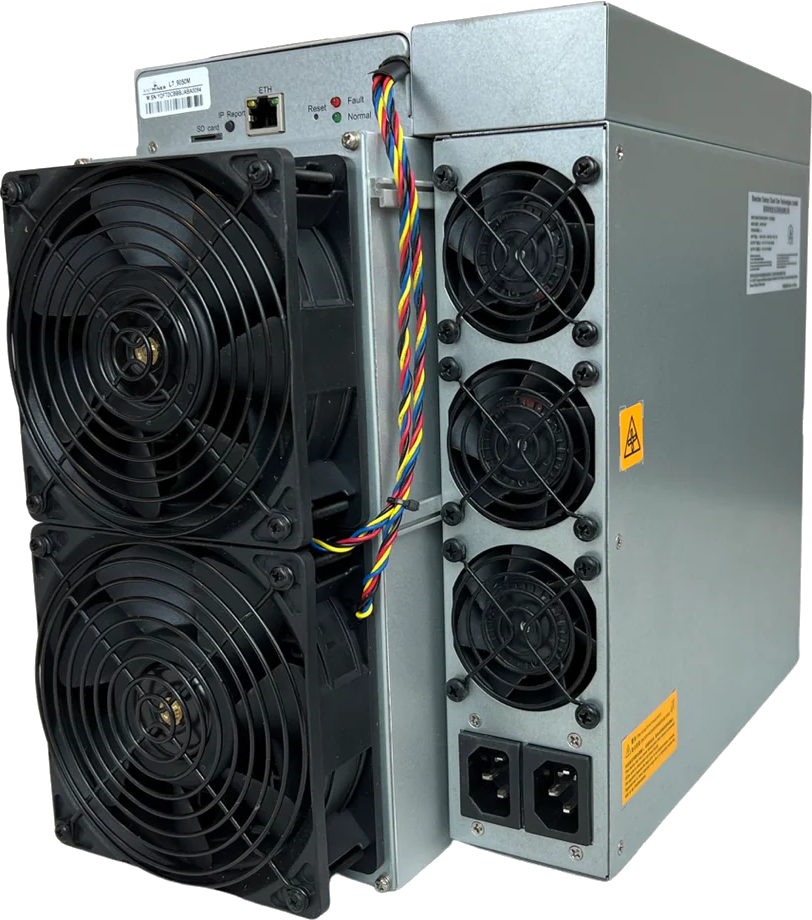
\includegraphics{img/antminer.png}
        }

        \caption{Un mineur Antminer L7}
      \end{figure}
    \end{column}
    \begin{column}{0.1\textwidth}\end{column}
  \end{columns}
\end{frame}

\begin{frame}{Frais de transaction}
  Émettre une transaction sur une blockchain n'est jamais gratuit et se paye en BTC.

  \begin{figure}
  \begin{tikzpicture}
    \begin{axis}[
        width=0.9\textwidth,
        height=6cm,
        grid = major,
        grid style={dashed, gray!30},
        date coordinates in=x,
        enlarge x limits=false,
        xtick distance=90,
        xticklabel={\month-\year},
      ]
      \addplot[myuniversity] table [x=date, y=tx_fee, col sep=comma] {data/btc-tx-fee.csv};
    \end{axis}
  \end{tikzpicture}
\end{figure}
\end{frame}